%(BEGIN_QUESTION)
% Copyright 2006, Tony R. Kuphaldt, released under the Creative Commons Attribution License (v 1.0)
% This means you may do almost anything with this work of mine, so long as you give me proper credit

Beregn følgende spenningsfall i kretsen under, gitt termoelementspiss-temperatur 718$^{o}$ F, perfekt kalibrering av øvrige instrumenter i sløyfen (temperaturområde = 500 til 1000$^{o}$ F; strømområde = 4 til 20 mA), og DC-forsyning på nøyaktig 28 volt:

$$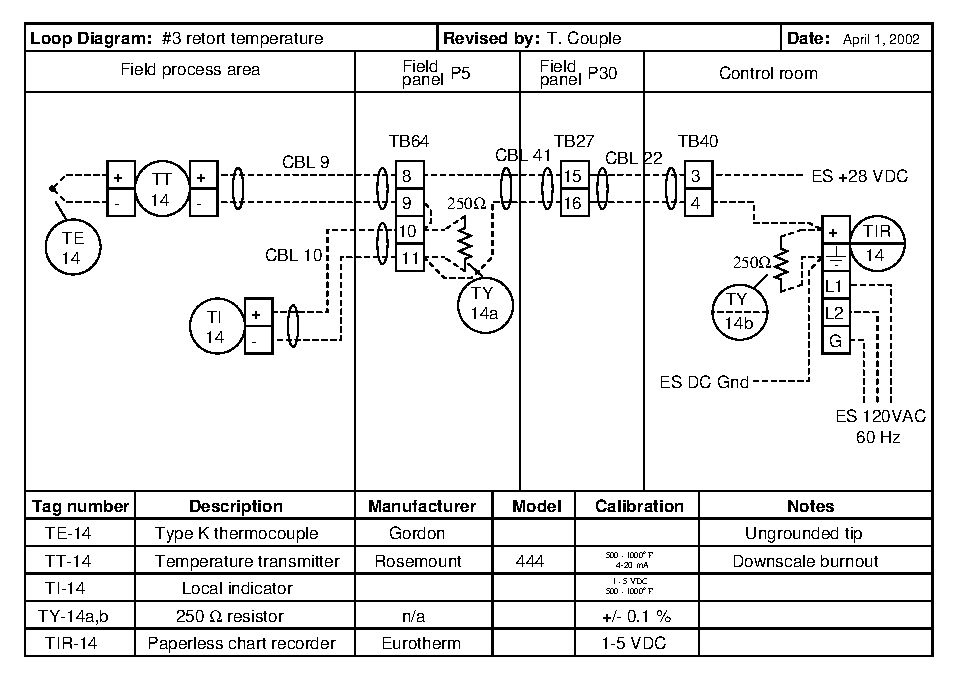
\includegraphics[width=15.5cm]{i00393x01.eps}$$

\begin{itemize}
\item{} Spenning mellom TB64-8 og TB64-9 =
\vskip 5pt
\item{} Spenning mellom TB64-10 og TB64-11 =
\vskip 5pt
\item{} Spenning mellom TB27-15 og TB27-16 =
\end{itemize}

\vskip 10pt

Bestem også hvor en {\it loop-kalibrator} kan kobles inn for å erstatte transmitteren, og hvilken modus kalibratoren må stå i for å styre sløyfestrømmen.

\vskip 20pt \vbox{\hrule \hbox{\strut \vrule{} {\bf Forslag til sokratisk diskusjon} \vrule} \hrule}

\begin{itemize}
\item{} Vis hvordan du kan {\it anslå} svarene uten kalkulator.
\item{} Diskuter mulige termoelementspisstyper, og sammenlign denne spissens egenskaper med andre.
\item{} Forklar hva ``downscale burnout'' betyr, og hvorfor denne transmitterkonfigurasjonen kan være viktig.
\item{} Hva er en ``paperless'' skriver/registrator?
\item{} Hva skjer i systemet dersom lokalindikatoren (TI-14) feiler åpen krets?
\end{itemize}

\underbar{file i00393}
%(END_QUESTION)





%(BEGIN_ANSWER)

\begin{itemize}
\item{} Spenning mellom TB64-8 og TB64-9 = 22.512 volt
\vskip 5pt
\item{} Spenning mellom TB64-10 og TB64-11 = 2.744 volt
\vskip 5pt
\item{} Spenning mellom TB27-15 og TB27-16 = 25.256 volt
\end{itemize}

\vskip 10pt

Hint: Hvis kretsanalysen er vanskelig, tegn kretsen om i skjematisk form (alle strømbærende komponenter i rett linje for å vise serieforbindelser).

%(END_ANSWER)





%(BEGIN_NOTES)

En loop-kalibrator kan settes i ``Simulate''-modus og kobles der transmitteren var (etter frakobling av transmitteren). Alternativt kan sløyfen brytes og kalibratoren brukes til å ``Source'' strøm direkte til 250 ohm-motstanden.






\filbreak \vskip 20pt \vbox{\hrule \hbox{\strut \vrule{} {\bf Virtuell feilsøking} \vrule} \hrule}

\noindent
{\bf Forutsi effekt av gitt feil:} presenter hver feil under for studentene, én om gangen, og la dem kommentere alle effekter hver feil vil gi.

\begin{itemize}
\item{}
\item{}
\item{}
\end{itemize}


\vskip 10pt


\noindent
{\bf Identifisere mulige/umulige feil:} presenter symptomer og la studentene avgjøre om foreslåtte feil kan forklare alle symptomene, med forklaring {\it hvorfor} eller {\it hvorfor ikke}:

\begin{itemize}
\item{} Symptom: {\it Anta at TIR-14 viser under 500 grader F}
\item{} TY-14a-motstand med brudd -- {\bf Ja}
\item{} TY-14a-motstand kortsluttet -- {\bf Nei}
\item{} TY-14b-motstand med brudd -- {\bf Nei}
\item{} TY-14b-motstand kortsluttet -- {\bf Ja}
\item{} TE-14 med brudd -- {\bf Ja}
\item{} TE-14 kortsluttet -- {\bf Ja}
\item{} Kabel CBL9 med brudd -- {\bf Ja}
\item{} Kabel CBL9 kortsluttet -- {\bf Nei}
\item{} Kabel CBL22 med brudd -- {\bf Ja}
\item{} Kabel CBL22 kortsluttet -- {\bf Nei}
\end{itemize}


\vskip 10pt


\noindent
{\bf Vurdere nytte av diagnostiske tester:} presenter symptomer og foreslå testene under én og én. Studentene vurderer om testen gir nyttig informasjon (altså noe vi ikke visste fra før), og hva ulike testresultater betyr:

\begin{itemize}
\item{} Symptom: {\it }
\item{}  -- {\bf Ja/Nei}
\item{}  -- {\bf Ja/Nei}
\end{itemize}


\vskip 10pt


\noindent
{\bf Diagnostiser feil fra gitte symptomer:} tenk deg at ??? feiler ??? i dette systemet (ikke avslør feilen). Presenter operatørobservasjon(er), la studentene foreslå feil og teststrategi, og oppgi testresultater de ber om til de har identifisert feiltype og plassering korrekt:

\begin{itemize}
\item{} Operatørobservasjon: {\it }
\item{}
\item{}
\end{itemize}
%INDEX% Basics, loop-powered transmitter: voltage drop calculations
%INDEX% Documentation, loop diagram

%(END_NOTES)
